\chapter{Strided Access, B-Trees, and the Impact of Virtual Paging}
\label{cha:lecture-two}

\begin{center}
  \textbf{Lecture 2}\\
  \emph{Strided access, binary search versus B-Trees, and virtual paging}\\[0.5em]
  Date: September 16, 2026
\end{center}

This chapter studies how an algorithm's access pattern interacts with the
transfer granularity of a memory system. The same arithmetic work can have
very different costs depending on whether accesses preserve spatial locality,
match the block size, or exceed the capacity of fast memory.

\section{Non-Sequential Access: The \texorpdfstring{$A_{s,b}$}{A-s-b} Algorithm}
\label{sec:strided-access}

Let $S$ be an array containing $n$ elements. The storage system transfers data
in physical blocks of size $B$ (a disk block or cache line). We also define a
logical block size $b$, where $b \leq B$ and $b$ divides $B$. The corresponding
numbers of logical and physical blocks are
\[
  N' = \frac{n}{b},
  \qquad
  N_{\mathrm{phys}} = \frac{n}{B}.
\]

The algorithm $A_{s,b}$ computes the sum of the elements by visiting logical
blocks in a stride pattern. The logical block visited at step $j$ is
\[
  \operatorname{block}(j) = (j s) \bmod N',
  \qquad j = 0,1,\ldots,N'-1.
\]

\subsection{Coprimality Condition}
\label{subsec:coprimality}

The sequence visits every logical block exactly once if and only if
\[
  \gcd\!\left(s,\frac{n}{b}\right)=1.
\]
In that case, multiplication by $s$ is a permutation of the residues modulo
$N'$. If the greatest common divisor is $d>1$, the sequence repeats after
$N'/d = n/(bd)$ distinct logical blocks and therefore covers only a fraction
of the array.

\begin{figure}[htbp]
  \centering
  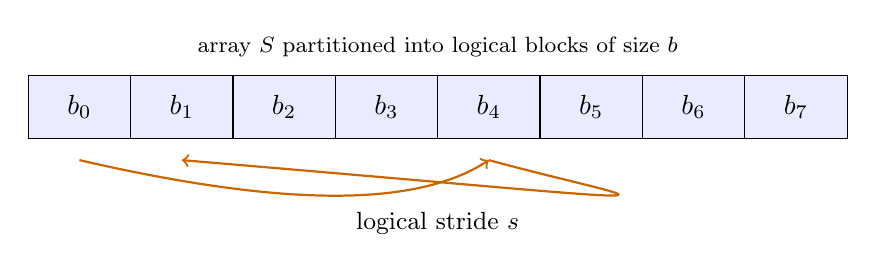
\begin{tikzpicture}[x=13mm,y=8mm]
    \foreach \i in {0,...,7} {
      \draw[fill=blue!8] (\i,0) rectangle ++(1,1);
      \node at (\i+0.5,0.5) {$b_{\i}$};
    }
    \draw[->,thick,orange!80!black] (0.5,-0.35) .. controls (2.5,-1.1) and (3.8,-1.1) .. (4.5,-0.35);
    \draw[->,thick,orange!80!black] (4.5,-0.35) .. controls (6.2,-1.1) and (7.0,-1.1) .. (1.5,-0.35);
    \node[font=\small] at (4,-1.35) {logical stride $s$};
    \node[font=\footnotesize,align=center] at (4,1.45)
      {array $S$ partitioned into logical blocks of size $b$};
  \end{tikzpicture}
  \caption{A modular stride visits logical blocks in a non-sequential order.}
  \label{fig:logical-stride}
\end{figure}

\autoref{fig:logical-stride} illustrates the logical access order. The
physical cost depends on how this order maps to blocks of size $B$, rather
than only on the number of arithmetic operations.

\subsection{I/O Cost}
\label{subsec:stride-io}

A useful first approximation compares the physical distance between successive
logical accesses, $s b$, with the physical block size $B$.

\begin{table}[htbp]
  \centering
  \caption{Approximate I/O behavior of the strided access pattern.}
  \label{tab:stride-io}
  \begin{tabularx}{\textwidth}{@{}p{0.25\textwidth}YY@{}}
    \toprule
    Condition & Locality and behavior & I/O cost \\
    \midrule
    $s b < B$ & Several logical accesses can share one physical block; partial
      spatial locality is preserved. & $\Theta(n/B)$ \\
    $s b \geq B$ & Successive accesses typically fall on different physical
      blocks. If $M<n$, the working set cannot remain entirely in fast memory. &
      $\Theta(n/b)$ \\
    $b=1$ and $s\geq B$ & Each logical access is one element and the stride
      destroys the benefit of block transfers. & $\Theta(n)$ \\
    \bottomrule
  \end{tabularx}
\end{table}

The bounds in \autoref{tab:stride-io} describe the usual worst-case or
capacity-miss regime. Exact constants depend on alignment, replacement policy,
and the interaction between the modular sequence and physical blocks. In the
last case, the cost is a factor of roughly $B$ worse than a linear scan, which
can exploit every transferred element.

\section{Algorithmic Limits and Hardware Acceleration}
\label{sec:scaling-laws}

Fix a maximum admissible execution time $T_0$ and assume that hardware or
parallelism accelerates the computation by a factor $K$. The accelerated
machine can therefore afford an original running time of
\[
  \frac{T(n)}{K}=T_0
  \qquad\Longleftrightarrow\qquad
  T(n)=K T_0.
\]
The effect on the largest solvable input depends on the growth rate of $T$.

\begin{table}[htbp]
  \centering
  \small
  \caption{Effect of a $K$-fold hardware acceleration on solvable input size.}
  \label{tab:scaling-laws}
  \begin{tabularx}{\textwidth}{@{}p{0.15\textwidth}p{0.19\textwidth}YY>{\raggedright\arraybackslash}p{0.18\textwidth}@{}}
    \toprule
    Algorithm & Complexity & Base hardware & Accelerated hardware & Effective gain \\
    \midrule
    $A_1$ & $c n$ & $n_1=T_0/c$ & $n'_1=K n_1$ & Multiplicative, $K$ \\
    $A_2$ & $c n^2$ & $n_2=\sqrt{T_0/c}$ & $n'_2=\sqrt{K}\,n_2$ & Sublinear, $\sqrt K$ \\
    $A_3$ & $c2^n$ & $n_3=\log_2(T_0/c)$ & $n'_3=n_3+\log_2 K$ & Additive, $+\log_2 K$ \\
    \bottomrule
  \end{tabularx}
\end{table}

\begin{figure}[htbp]
  \centering
  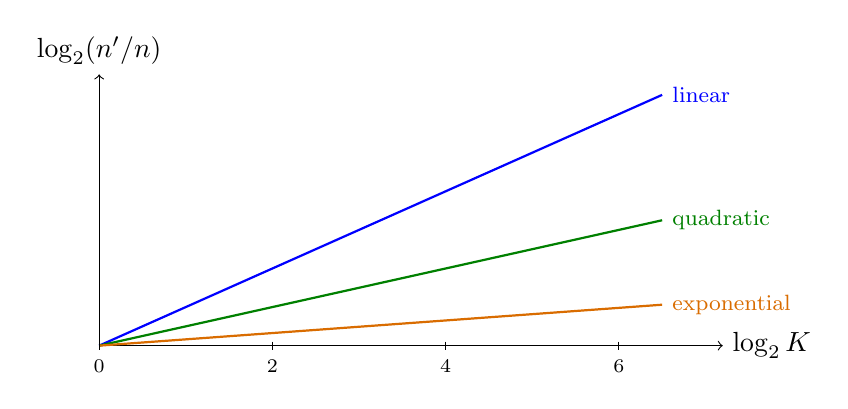
\begin{tikzpicture}[x=1.1cm,y=0.65cm]
    \draw[->] (0,0) -- (7.2,0) node[right] {$\log_2 K$};
    \draw[->] (0,0) -- (0,5.3) node[above] {$\log_2(n'/n)$};
    \draw[thick,blue] (0,0) -- (6.5,4.9) node[right,font=\footnotesize] {linear};
    \draw[thick,green!50!black] (0,0) -- (6.5,2.45) node[right,font=\footnotesize] {quadratic};
    \draw[thick,orange!85!black] (0,0) -- (6.5,0.8) node[right,font=\footnotesize] {exponential};
    \foreach \x/\label in {0/0,2/2,4/4,6/6} {
      \draw (\x,0.08) -- (\x,-0.08) node[below,font=\scriptsize] {\label};
    }
  \end{tikzpicture}
  \caption{Relative benefit of hardware acceleration for representative growth rates.}
  \label{fig:scaling-laws}
\end{figure}

\autoref{fig:scaling-laws} shows why hardware improvements do not remove an
asymptotically inefficient algorithm. For an exponential algorithm, even a
$1000$-fold speedup increases the solvable input size by only
$\log_2(1000)\approx 10$ elements.

\section{Searching Ordered Sets: Binary Search versus B-Trees}
\label{sec:binary-search-btrees}

\subsection{Binary Search in Secondary Memory}
\label{subsec:external-binary-search}

For a sorted sequence of $n$ keys stored in blocks of size $B$, binary search
performs $\Theta(\log_2 n)$ comparisons on the CPU. Its I/O cost is larger
than its comparison count suggests: during the first iterations, the examined
positions are separated by $n/2$, $n/4$, and so on. Until the search interval
shrinks to at most $B$ elements, each probe can address a different physical
block. Thus,
\[
  \operatorname{I/O}_{\mathrm{binary\ search}}
  \approx \log_2 n-\log_2 B
  = \log_2\!\left(\frac{n}{B}\right).
\]
The approximation ignores alignment and the possibility that a block remains
cached, but captures the dominant external-memory behavior.

\subsection{B-Trees and \texorpdfstring{B$^+$-Trees}{B+-Trees}}
\label{subsec:btree}

A B-Tree chooses the node size to match one physical block. Each node stores
$\Theta(B)$ keys and child pointers, so its fan-out is $\Theta(B)$. A B$^+$-Tree
uses the same principle and normally stores records or record pointers in its
leaves, making it especially suitable for range queries.

\begin{figure}[htbp]
  \centering
  \begin{tikzpicture}[
    nodebox/.style={draw,rounded corners=2pt,minimum height=8mm,align=center,font=\small},
    edge/.style={-Latex,thick},
    level distance=13mm,
    sibling distance=27mm
  ]
    \node[nodebox,fill=blue!12] (root) {[K$_1$ \textbar K$_2$ \textbar K$_3$]\\root block};
    \node[nodebox,fill=green!10,below left=of root] (left) {child block};
    \node[nodebox,fill=green!10,below=of root] (middle) {child block};
    \node[nodebox,fill=green!10,below right=of root] (right) {child block};
    \draw[edge] (root) -- (left);
    \draw[edge] (root) -- (middle);
    \draw[edge] (root) -- (right);
    \node[font=\footnotesize,below=7mm of middle] {each node occupies approximately one physical block $B$};
  \end{tikzpicture}
  \caption{A block-oriented B-Tree with high fan-out.}
  \label{fig:btree}
\end{figure}

\autoref{fig:btree} shows the central layout decision: one I/O loads an entire
node and supplies many routing keys and pointers. The height, and therefore
the number of block reads for a point query, is approximately
\[
  h = \log_B\!\left(\frac{n}{B}\right)
    = \frac{\log_2(n/B)}{\log_2 B}.
\]
More precisely, implementation details introduce ceilings and occupancy
factors. The internal-node space is small compared with the leaves because
\[
  \text{internal nodes}
  \leq \frac{n}{B^2}+\frac{n}{B^3}+\cdots
  = \frac{n}{B(B-1)}
  \ll \frac{n}{B}.
\]

\subsection{Quantitative Comparison}
\label{subsec:btree-comparison}

Ignoring ceilings, the I/O speedup of a B-Tree over binary search is
\[
  \frac{\operatorname{I/O}_{\mathrm{binary\ search}}}
       {\operatorname{I/O}_{\mathrm{B\text{-}Tree}}}
  = \frac{\log_2(n/B)}{\log_2(n/B)/\log_2 B}
  = \log_2 B.
\]

\begin{table}[htbp]
  \centering
  \caption{Illustrative comparison for a large ordered dataset.}
  \label{tab:btree-example}
  \begin{tabularx}{\textwidth}{@{}lX@{}}
    \toprule
    Parameter & Value \\
    \midrule
    Dataset size & $n=2^{40}$ elements, approximately $10^{12}$ records \\
    Block size & $B=2^{14}=16\,384$ records \\
    Binary-search I/O & $40-14=26$ block accesses \\
    B-Tree I/O & $(40-14)/14\approx1.85$, hence about $2$ block accesses \\
    \bottomrule
  \end{tabularx}
\end{table}

For millisecond-scale storage latency, the difference between approximately
$26$ and $2$ block accesses changes a point query from hundreds of milliseconds
to only a few milliseconds, subject to caching and hardware details.

\section{I/O-Aware Algorithms and Virtual Paging}
\label{sec:paging}

There are two complementary ways to manage transfers between fast and slow
memory:

\begin{description}
  \item[I/O-aware design (explicit).] The algorithm models $B$ and the fast
    memory capacity $M$ directly, and manages buffers, data layout, and
    transfers programmatically.
  \item[Virtual memory and paging (implicit).] The operating system and the
    hardware transparently move pages using page tables and replacement
    policies such as LRU approximations.
\end{description}

\subsection{Paging with an Oversized Working Set}
\label{subsec:paging-model}

Assume that physical memory has capacity $M$ and is divided into $M/B$ frames.
If the application requires
\[
  n=(1+\varepsilon)M=M+\varepsilon M,
  \qquad \varepsilon>0,
\]
then at least $\varepsilon M$ units of the working set must reside in
secondary storage. Let $\alpha$ be the fraction of instructions that perform
memory operations. A typical instruction profile is:

\begin{itemize}
  \item fraction $1-\alpha$: arithmetic or logical operations, with cost
    approximately one CPU cycle;
  \item fraction $\alpha$: `LOAD` or `STORE` operations;
  \item probability $1-P(\varepsilon)$: the referenced data are resident in
    RAM, with access time $t_m$;
  \item probability $P(\varepsilon)$: the access causes a page fault, with
    service time $t_{\mathrm{disk}}$.
\end{itemize}

The resulting average time per instruction is
\[
  T_{\mathrm{avg}}=(1-\alpha)\cdot1
  +\alpha\left[(1-P(\varepsilon))t_m
  +P(\varepsilon)t_{\mathrm{disk}}\right].
\]
Since $t_m\ll t_{\mathrm{disk}}$, the page-fault term can dominate:
\[
  T_{\mathrm{avg}}\approx
  \alpha P(\varepsilon)t_{\mathrm{disk}}.
\]
This approximation is a warning about sensitivity, not an identity: when
$P(\varepsilon)$ is zero, the baseline CPU and RAM terms still matter.

\subsection{Numerical Thrashing Example}
\label{subsec:thrashing}

Take $\alpha=0.3$, a page-fault penalty of
$t_{\mathrm{disk}}=10^5$ clock cycles, and a fault probability of only
$P(\varepsilon)=10^{-3}$. Then the expected penalty is
\[
  T_{\mathrm{penalty}}
  \approx 0.3\cdot10^{-3}\cdot10^5
  =30\text{ cycles per instruction}.
\]
One page fault every thousand memory accesses can therefore add about $30$
cycles to every instruction on average. Relative to a one-cycle baseline,
this can produce an order-of-magnitude slowdown, potentially in the
$10\times$--$30\times$ range depending on the ordinary RAM latency and the
actual working-set behavior. When the fault rate rises further, the process
enters \emph{thrashing}: the system spends most of its time servicing page
faults instead of progressing with useful computation.

\section{Key Takeaways}
\label{sec:lecture-two-takeaways}

\begin{enumerate}
  \item A modular stride visits all logical blocks only when the stride and the
    number of logical blocks are coprime.
  \item Block-aware layouts and access patterns can change I/O complexity by a
    factor of $B$, even when CPU work is unchanged.
  \item B-Trees reduce external-memory search depth by matching their fan-out
    to the physical block size.
  \item Hardware acceleration improves linear and polynomial algorithms in
    different ways, but gives only an additive improvement to exponential
    algorithms.
  \item Virtual memory is convenient, but an oversized working set can turn a
    small page-fault probability into a dominant performance cost.
\end{enumerate}
